\chapter{绪论}

\section{研究背景与意义}

\subsection{研究背景}

目前,世界仍在与新冠病毒作斗争,世界正处于大变革、大调整和两极分化的转折点。从目前疫情来看,即使一些国家实现了所谓的“群体免疫”,但除中国、韩国、朝鲜和新西兰等少数国家外,大多数国家的社会开放和经济重启计划仍远未达到预期。一些医学专家甚至断言,COVID-19将与人类长期共存。在此之前,由于中美之间的结构性竞争和贸易摩擦,全球经济地理空间重组。COVID-19的爆发无疑加剧了中美之间固有的差异。疫情发生后,世界格局将迎来新一轮深刻调整,世界新秩序正在全球抗击疫情的斗争中悄然孕育。展望未来,以开放、包容、协作和协商为特征的全球安全进程可能会突然结束,取而代之的是全球供应链和产业链的中断、国家间人员交流的限制性孤立以及各种种族主义和仇外心理的抬头。在新的政治形势和新的技术环境下,大数据被广泛应用于新冠疫情防控和社会稳定监测。以新冠疫情防控为契机,以精准安全管理为目标,以大数据为核心动力,全球安全管理人工智能时代正在悄然开启。

2020年2月,世卫组织总干事谭德塞在记者会上宣布,将新型冠状病毒命名为“COVID-19”。据国家卫生委员会统计,截止2021年8月7日,我国31个省(区、市)和新疆建设兵团累计确诊病例121454例,累计死亡5654人;国外累计确诊病例202337884,累计死亡4285250人。我国国内确诊病例数仍呈现上升趋势,可见当前国内疫情形势仍然相当严峻。


\subsection{研究意义}

新型冠状病毒肺炎疫情在 2019 年底爆发,并迅速在全球范围内传播。疫情发展实况与每个人的工作和生活息息相关。同时,网络上也出现了疫情相关的虚假信息和谣言,扰乱了社会防疫抗疫秩序。基于爬虫编程技术实现了对新冠疫情数据的采集,通过疫情数据可视化,将国内外疫情形态以更直观的方式传递给大众,帮助人们更好地了解国内外疫情实况,提高防范意识,从而有效地协调、安排和开展各项工作和生活等。本系统使用Flask框架、Python构建轻量级疫情数据发布平台,将疫情数据转换为可视化的地图与表格,最大程度上满足疫情时代下人们的普遍需求。本文将从疫情数据的获取及存储、网页设计等几个方面进行阐述。\citep{李宏2020基于民众视阈下的疫情数据可视化设计路径研究}

2020年初,新型冠状病毒肺炎疫情已成为世界焦点,从疫情初现端倪,政府和企业在此次疫情中的数据可视化,让公众直观地掌握疫情动态。达到防控风险,抑制疫情的再扩散的目的。当今世界已经进入大数据时代,各国已将数据列为新的战略资源。在经济高速运转的今天,数据不再局限于小小的一个圈子,而是更加开放、包容,数据规模也更为客观。数据不再是简单的数字,如何从数据的背后挖掘出数据潜藏的价值成为国家和企业关心的热点问题。\citep{郭宏曦2020新型冠状病毒肺炎疫情数据的可视化探索}

\section{国外研究现状}

针对全球流行的新型冠状病毒,Google新闻推出基于维基百科以及其他数据来源的疫情数据监测平台。世卫组织(WHO)也在其官网发布疫情数据以及预防感染措施,以减少人们对新冠病毒的恐惧。

\begin{figure}[H]
    \centering
    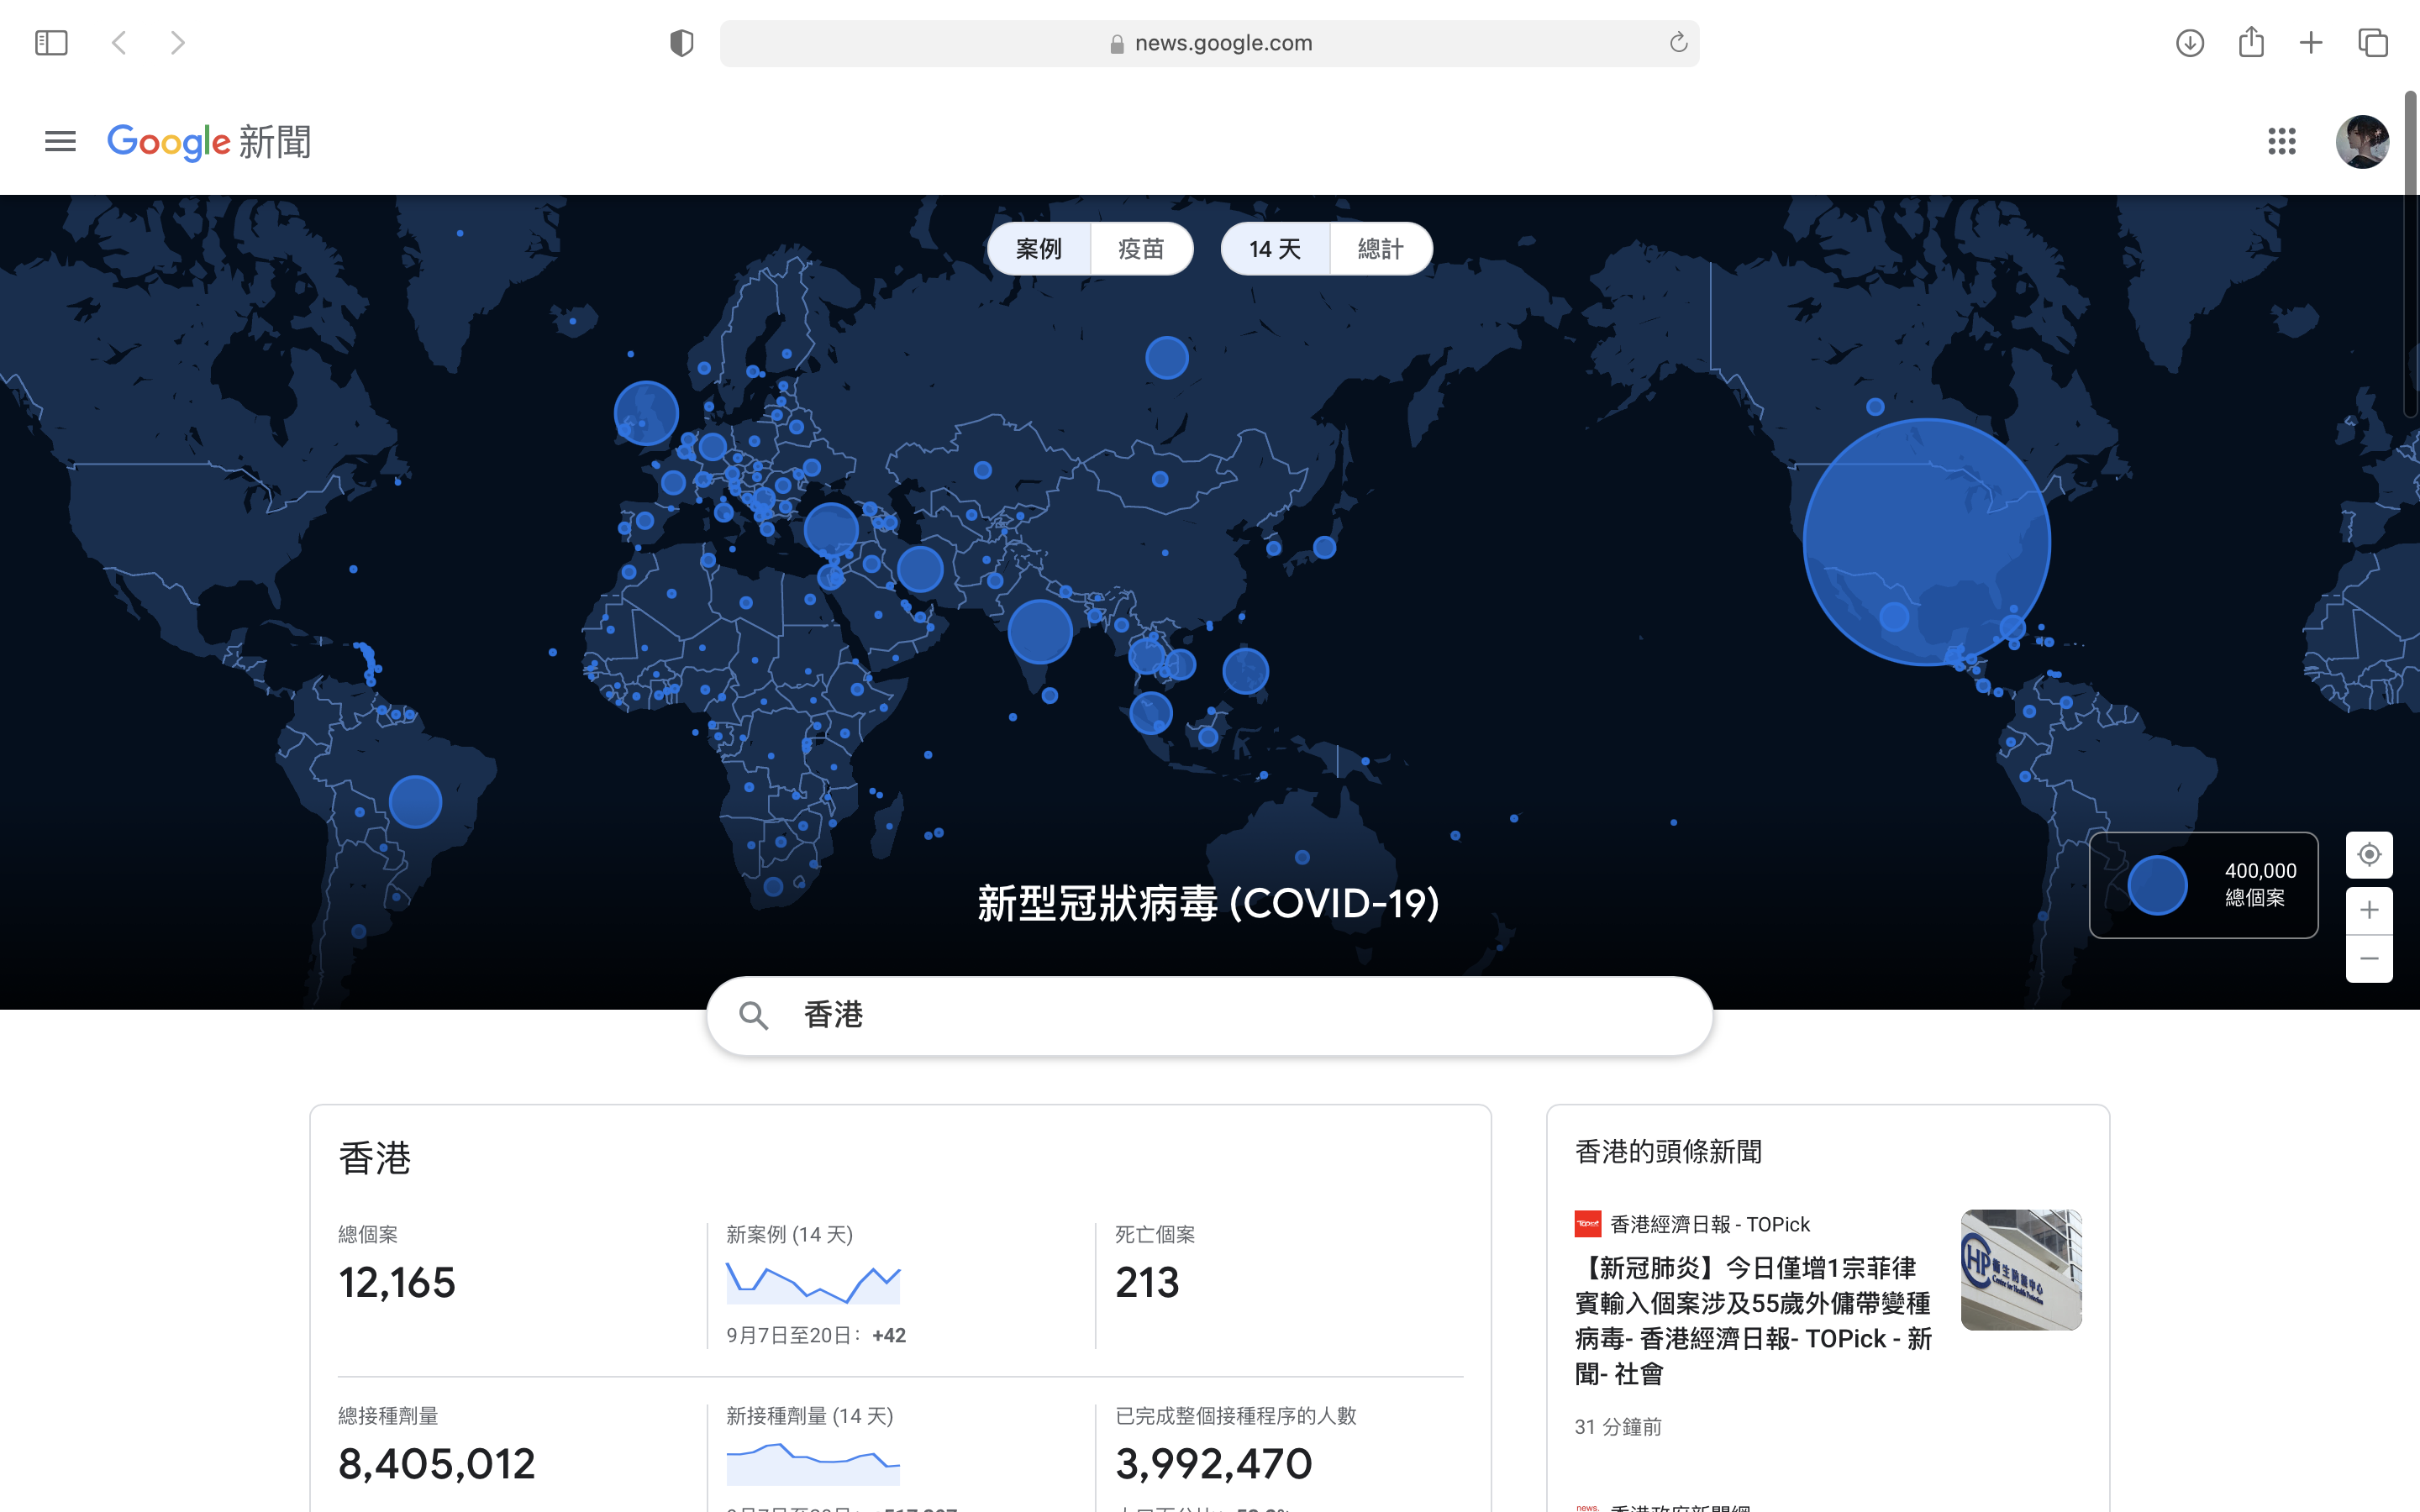
\includegraphics[width=0.8\textwidth]{t1}
    \bicaption{谷歌新闻疫情数据监测网站}{Google News epidemic data monitoring website}
    \label{fig:t1}
\end{figure}

\section{研究方法}

由于时间和精力的限制,本系统采用的疫情原始数据来自于阿里巴巴、腾讯或百度等已有疫情数据平台的数据源,而不再去统计疫情数据。

在现实生活中,单纯的数字不能直观地显示一段时间以来的发展状况,并且人脑对图像信息的处理能力也要优于对单纯数据的处理,所以将数据可视化更有利于普通大众更快地获取信息。同时,数据可能是多维度的,将数据按照一定规则分类、排序可视化之后更能清楚地看到数据的多维性,更能表达出数据与数据之间的关系。当前的数据可视化的系统设计方法有多种,但是主要的设计方法还是设计前端+后端+数据库的主体思路。\citep{韩洪勇2020基于}

基于Python+Echarts的大数据可视化系统采用B/S架构,借助于Python强大的数据获取和处理技术实现了区域网络餐饮数据的采集、清洗、整理及分析计算工作并推送至MySQL数据库中。后台采用基于Python的Flask框架实现数据接口功能,前端综合运用了HTML、CSS、JavaScript等,并结合Echarts数据可视化组件,实现了数据到可视化图表的转换。\citep{陈俊生2019基于}

